
\section{\rbt}

\vskip0.5cm

\subsection{ROTACIONES}

\begin{center}
		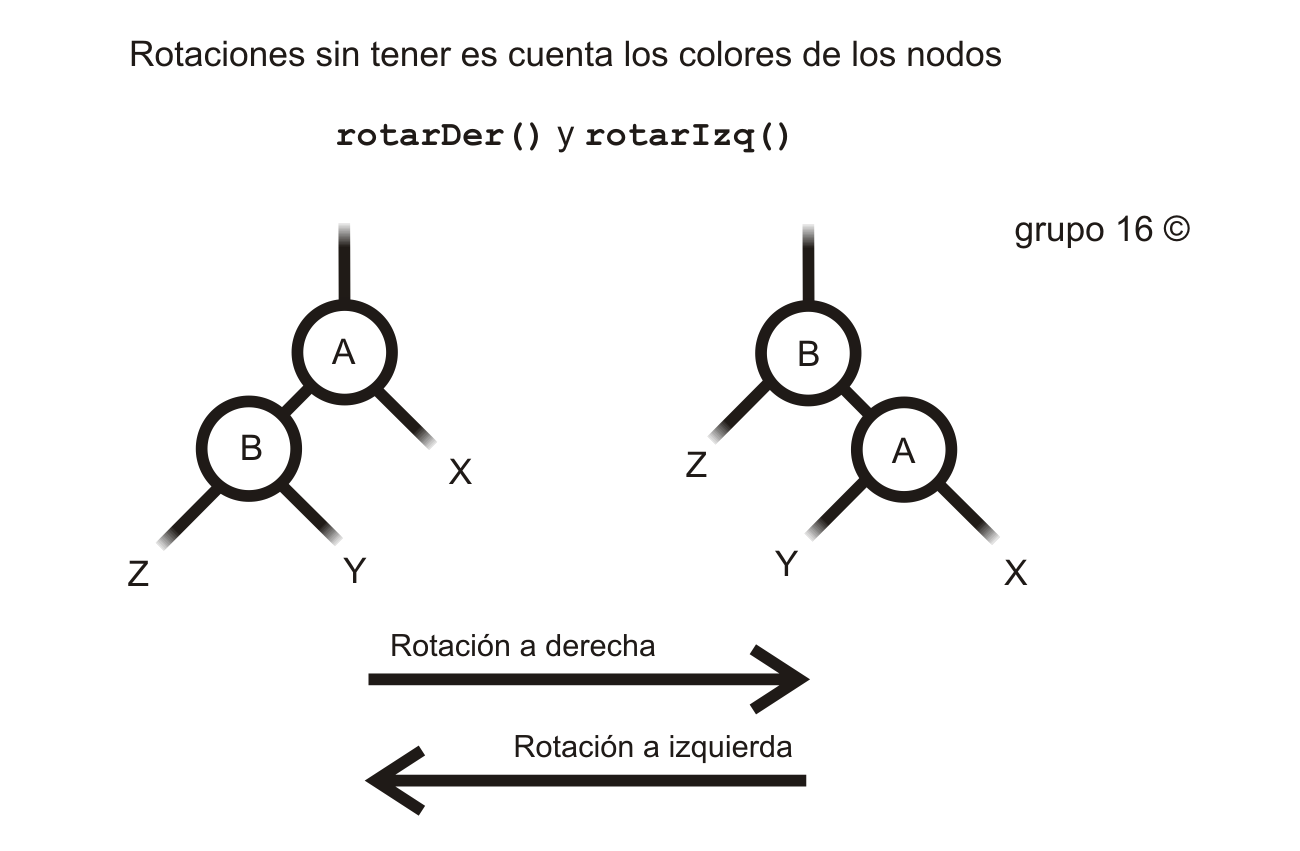
\includegraphics{rotaciones.png} \\
(figura 1.1)\\
\end{center}

Rotaciones simples para mantener el balanceo. (No son para hacerlo un AVL)

\subsection{CASO 1}

\begin{center}
		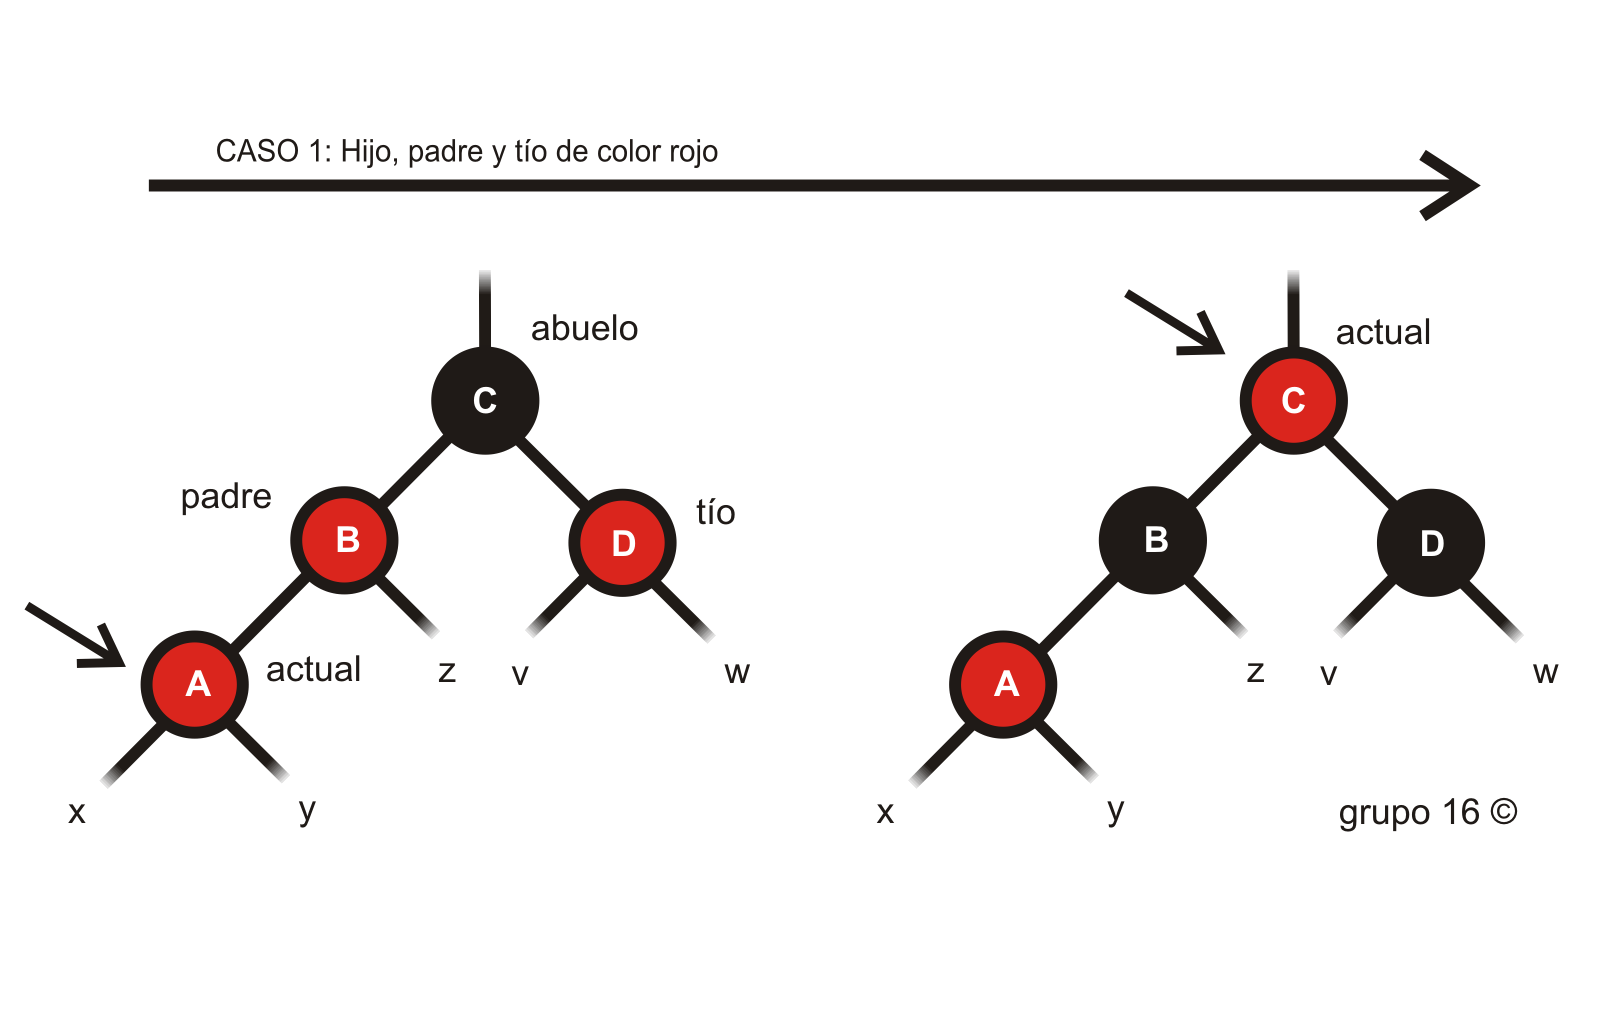
\includegraphics{caso1.png} \\
(figura 1.2)\\
\end{center}

Si A (Actual), B (Padre) y D (tio) son Rojos, estamos en \textsc{CASO 1}.\\
Pintamos al padre y tio de Negro, y pintamos a C (Abuelo) de Rojo. Como el arbol era un \rbt ese abuelo era negro.\\
Al hacer los cambios, alturas negras no se modifican. Por lo que hasta el abuelo tenemos todo arreglado.

\subsection{CASO 2}

\begin{center}
		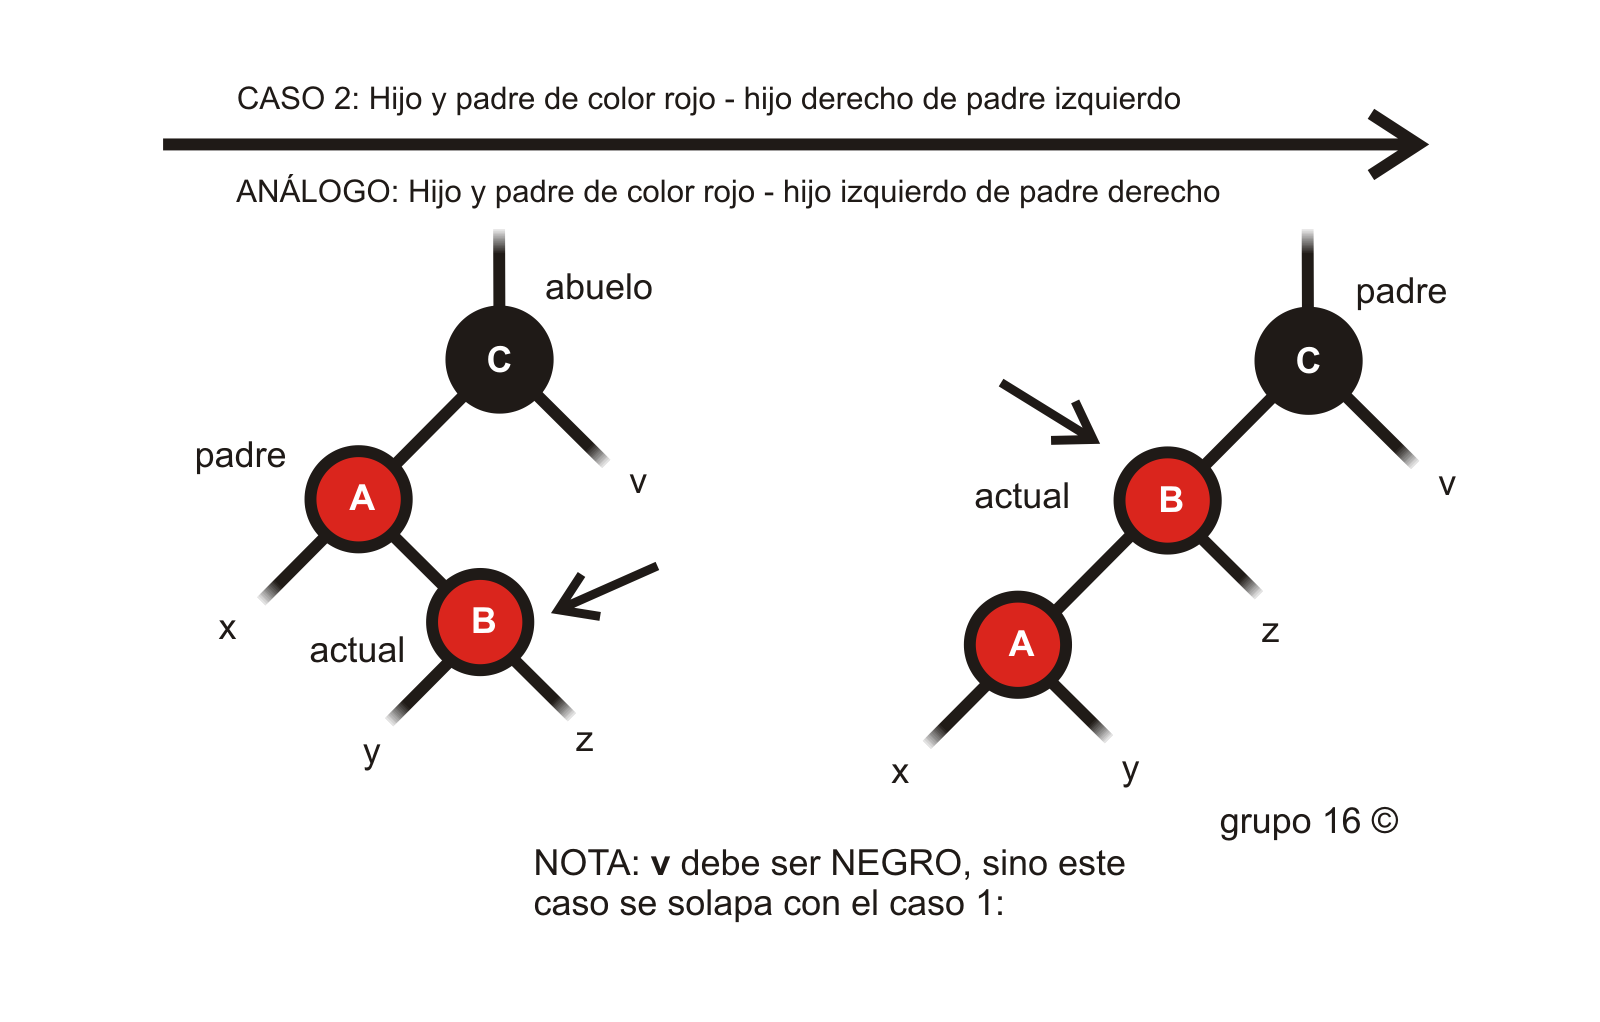
\includegraphics{caso2.png} \\
(figura 1.3)\\
\end{center}

Si B (Actual) y A (padre) son rojos y el tio es negro (o es nil - tambien considerado como regro) y ademas B es hijo derecho de un padre que es hijo izquierdo (o B es hijo izquierdo de un padre que es hijo derecho), estamos en \textsc{CASO 2}\\
Rotamos el padre a izquierda (o derecha segun el caso), y hemos reducido el \textsc{CASO 2} o un \textsc{CASO 3}.

\subsection{CASO 3}

\begin{center}
		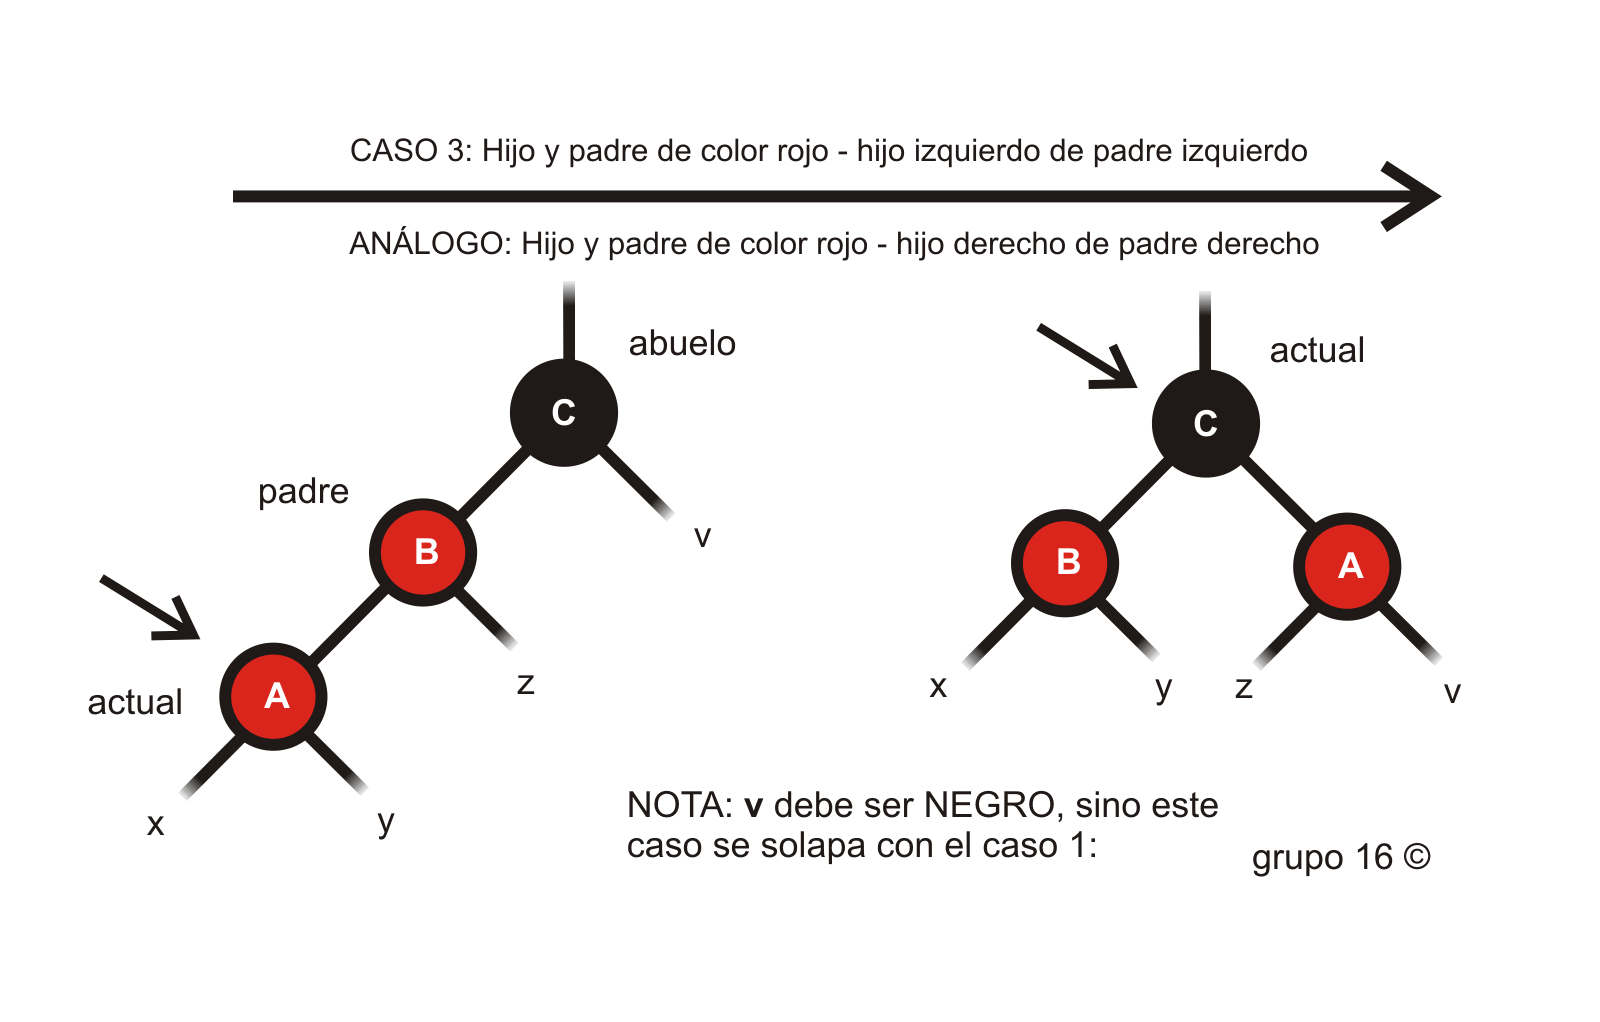
\includegraphics{caso3.png} \\
(figura 1.4)\\
\end{center}

Si A (Actual) y B (padre) son rojos y el tio es negro (o es nil - tambien considerado como regro) y ademas B es hijo derecho de un padre que es hijo derecho (o B es hijo izquierdo de un padre que es hijo izquierdo), estamos en \textsc{CASO 3}\\
Pintamos a padre negro, al abuelo rojo y y rotamos a derecha (o Izquerda segun el caso) al abuelo\\
Las alturas negras no se modifican y la posici�n del abuelo quedar�a negra, con ambos hijos rojo.

\subsection{TEST de Inserciones}

Hemos realizado un par de test para ``verificar'' el correcto fuincionemiento de las inserciones en el \rbt\\
Las inserciones fueron las siguientes $[10, 20, 15, 30, 40]$.\\
De esta manera probamos los casos mas interesantes:

\vskip0.3cm

\begin{tabular}{lll}
de $ninguno$ &			 a $[10]$ 					&	(CASO 0: Insertar raiz)\\
de $[10]$ &				 a $[10, 20]$				&	(CASO 0: Insertar con padres negro)\\
de $[10, 20]$ &			 a $[10, 20, 15]$ 			&	(CASO 2)\\
de $[10, 20, 15]$ &		 a $[10, 20, 15, 30]$ 		&	(CASO 1)\\
de $[10, 20, 15, 30]$ &	 a $[10, 20, 15, 30, 40]$ 	&	(CASO 3)\\
\end{tabular}
                                                                            
\vskip0.3cm

N�tese que en algunas de estas inserciones, \\
los llamados recursivos, llaman tambien a otros casos de ``reacomodacion''.\\
Para correr el test y observar la salida del programa se debe llamar al \verb|main| con parametro \verb|test|

\begin{center}
		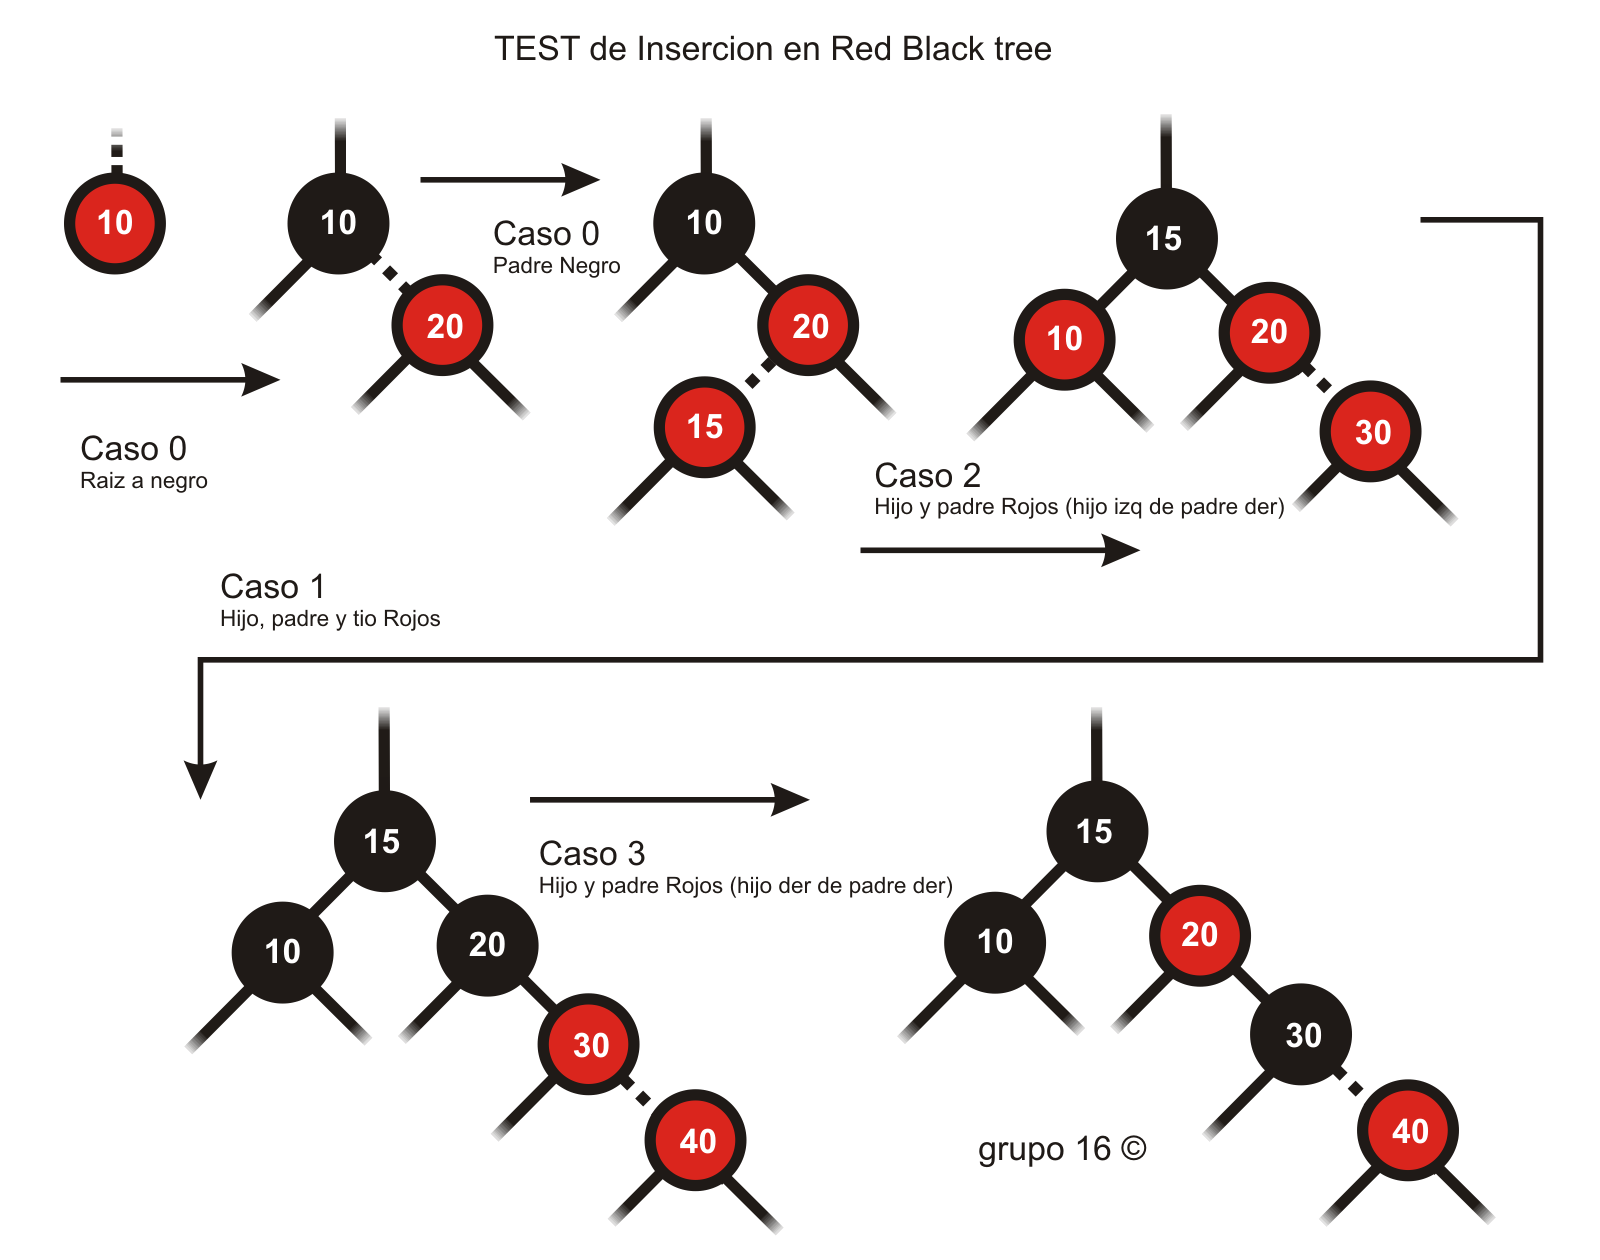
\includegraphics{test_insercion.png} \\
(figura 1.5)\\
\end{center}

\vskip0.5cm

\section{\adi}

\subsection{Ideas para la eleccion de estructura del \adi}

%//////////////////////////////////////////////////////////////////

\subsubsection{Dos �rboles}

La primera idea que se nos acurrio para extender el arbol de intervalos a dos dimenciones, fue simplemente tener dos �rboles (uno para cada coordenada).\\
La busqueda entonces consistia en buscar las imagenes correspondientes al la coordenada $x$ y luego las imagenes correspondientes a la coordenada $y$. Por ultimo, debiamos encontrar las imagenes que aparecieran en los dos conjuntos.

\vskip0.3cm

\Large Costo temporal de la construccion \normalsize

\vskip0.3cm

\Large Costo espacial de la construccion \normalsize

\vskip0.3cm

\Large Costo temporal total de la consulta \normalsize

\vskip0.3cm

\Large Costo espacial de la consulta  \normalsize

%//////////////////////////////////////////////////////////////////

\subsubsection{�rbol con ambas coordenadas}

Otra idea fue, hacer un solo arbol en el que los ``Intervalos Elementales'' se construyeran con todos los puntos de inicio y finalizacion de las coordenadas $x$ e $y$. En cada nodo de este arbol se encontrabas un arreglo (o alguna otra estructura) con las imagenes que le correspondian en $x$ y otro arreglo con las imagenes que le correspondian en $y$.\\
De esta manera teniamos un solo arbol y espacialmente reduciamos la cantidad de nodos existentes. (La cantidad de nodos con dos arboles era 

	\[\#\{IntervalosElementales(x)\} + \{IntervalosElementales(y)\}\]
	
y de esta manera era 

	\[\#(\{IntervalosElementales(x)\} \cup \{IntervalosElementales(y)\})\]

\vskip0.3cm

\Large Costo temporal de la construccion \normalsize

\vskip0.3cm

\Large Costo espacial de la construccion \normalsize

\vskip0.3cm

\Large Costo temporal total de la consulta \normalsize

\vskip0.3cm

\Large Costo espacial de la consulta \normalsize

%//////////////////////////////////////////////////////////////////

\subsubsection{�rboles dentro de �rbol}

...

\vskip0.3cm

\Large Costo temporal de la construccion \normalsize

\vskip0.3cm

\Large Costo espacial de la construccion \normalsize

\vskip0.3cm

\Large Costo temporal total de la consulta \normalsize

\vskip0.3cm

\Large Costo espacial de la consulta \normalsize


%//////////////////////////////////////////////////////////////////

\subsubsection{�rboles unico (en alguna de las dos coordenadas)}

...

\vskip0.3cm

\Large Costo temporal de la construccion \normalsize

\vskip0.3cm

\Large Costo espacial de la construccion \normalsize

\vskip0.3cm

\Large Costo temporal total de la consulta \normalsize

\vskip0.3cm

\Large Costo espacial de la consulta \normalsize

%//////////////////////////////////////////////////////////////////

\subsection{Conculciones sobre los algoritmos y eleccion}


\vskip0.5cm